%% Use the hmcposter class with the clinic document-class option.
\documentclass[thesis]{hmcposter}
\usepackage{graphicx}
\usepackage{natbib}
\usepackage{booktabs}
\usepackage{subfig}
\usepackage{amsmath}
\usepackage{textcomp}
\usepackage{url}

\usepackage{verbatim}

%% For a Clinic poster, there is no author (the author is the team).

%% Project Year.
%% The year is provided using the \year command.
\posteryear{2016}

%% Project Title.
%% The title of the poster should probably be the name of your
%% Clinic project.
%\title{User Experience and Feedback on the RPI Homework Submission Server}
\title{User Experience and Feedback on the\\
\vspace{-0.1in}
RPI Homework Submission Server}
%\author{Andrea Wong, Beverly Sihsobhon, Melissa Lindquist, Matt Peveler, Barbara Cutler, 
%Samuel Breese, Eric Tran, Joe Jung, Ben Shaw}
\author{Andrea Wong, Beverly Sihsobhon, Melissa Lindquist, Matt Peveler, Barbara Cutler, \\
\vspace{-0.7in}
Samuel Breese, Eric Tran, Joe Jung, Ben Shaw}

%%somehow cram names of the people going in under the title

%% Sponsor's Logo.
%% The name (base name only; no extension) of an image file with
%% the sponsor's logo.  Ideally, you'll have a PDF version that is
%% resolution-independent.  If not, you'll need a high-resolution
%% PNG file to allow us to print it at a large size without the
%% image becoming blurred.
\classlogo{lgplogo2cm}

%% Optional -- if your sponsor's logo looks too small or too big,
%% you can adjust its width with the \sponsorlogowidth command.
%% (The height of the logo image is automatically adjusted to
%% preserve the image's aspect ratio.)
%%
%% Note that the argument must be a TeX length; for example, 3in,
%% 5cm, 120pt, etc.  The default width is 2in.
\classlogowidth{2in}


%% Optional -- if your sponsor is hot about their intellectual
%% property and insists on having a copyright statement on the
%% poster, you can use the \copyrightholder command to supply a
%% name for a copyright holder for your poster.
% \copyrightholder{Sponsoring Corporation, Inc.}

\raggedcolumns

%% Define the \BibTeX command, used in our example document.
\providecommand{\bibtex}{{\rmfamily B\kern-.05em%
    \textsc{i\kern-.025em b}\kern-.08em%
    T\kern-.1667em\lower.7ex\hbox{E}\kern-.125emX}}


\pagestyle{fancy}

\begin{document}

\begin{poster}

\section{1. Introduction}
% Note that we're not labeling sections because you shouldn't be
% doing a lot of referring back and forth in your poster---let the
% interested folks read your thesis or Clinic report, or ask
% questions.

The Rensselaer Polytechnic Institute (RPI) Homework Submission Server
is an ongoing project of the Rensselaer Center for Open Source
Software (RCOS). The system collects, compiles, and automatically
grades the programming homeworks for students in our introductory,
sophomore, and upper division computer science classes.  Our research
has found that an electronic submission server is the preferred way
for students to submit their coding homeworks because it provides
immediate feedback about the correctness of their code and ensures
fair and consistent grading across all students in the course.

\begin{center}
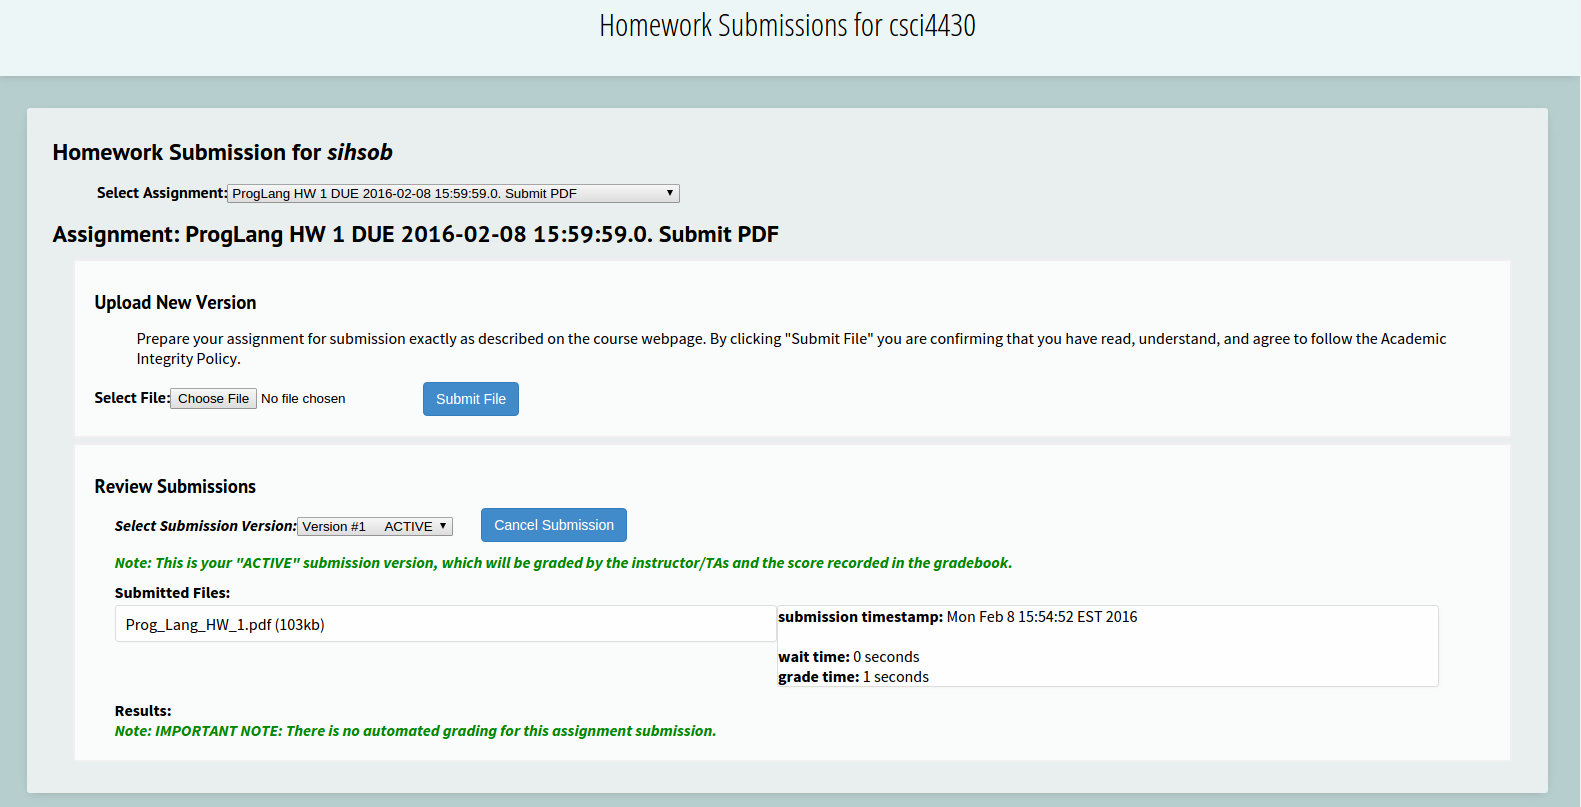
\includegraphics[width=12in]{HSS_prog_lang}
\end{center}

\begin{center}
    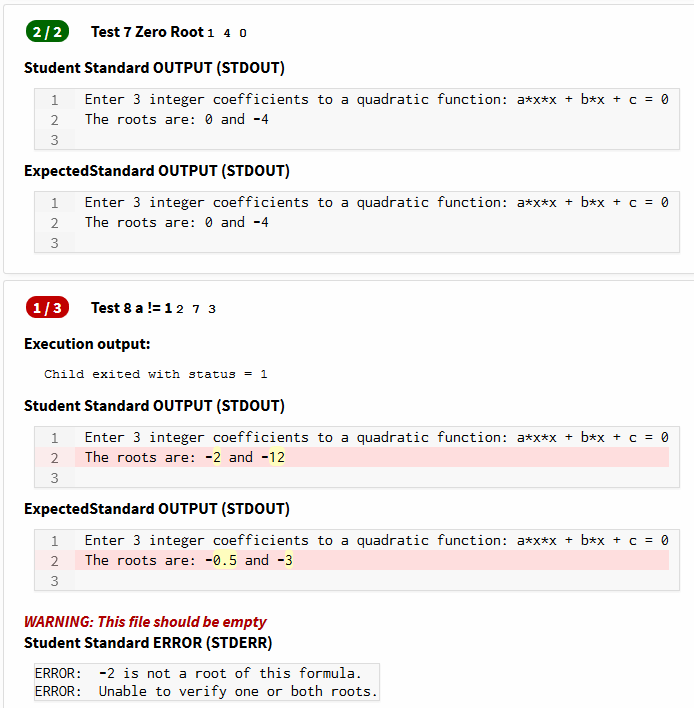
\includegraphics[width=12in]{PartialCredit}
\end{center}




\columnbreak

\section{2. System Features}%


\begin{itemize}
    \item Website for students to submit assignments and view results
    \item Automated testing and grading with immediate feedback
    \item View TA grade and comments on each homework
    \item Ability to make multiple submissions to the same homework
    \item Server accepts single file, zip file, or SVN repository submissions
    \item Highlight differences in the output produced by student's code \\ vs. the expected output
\end{itemize}

\begin{center}
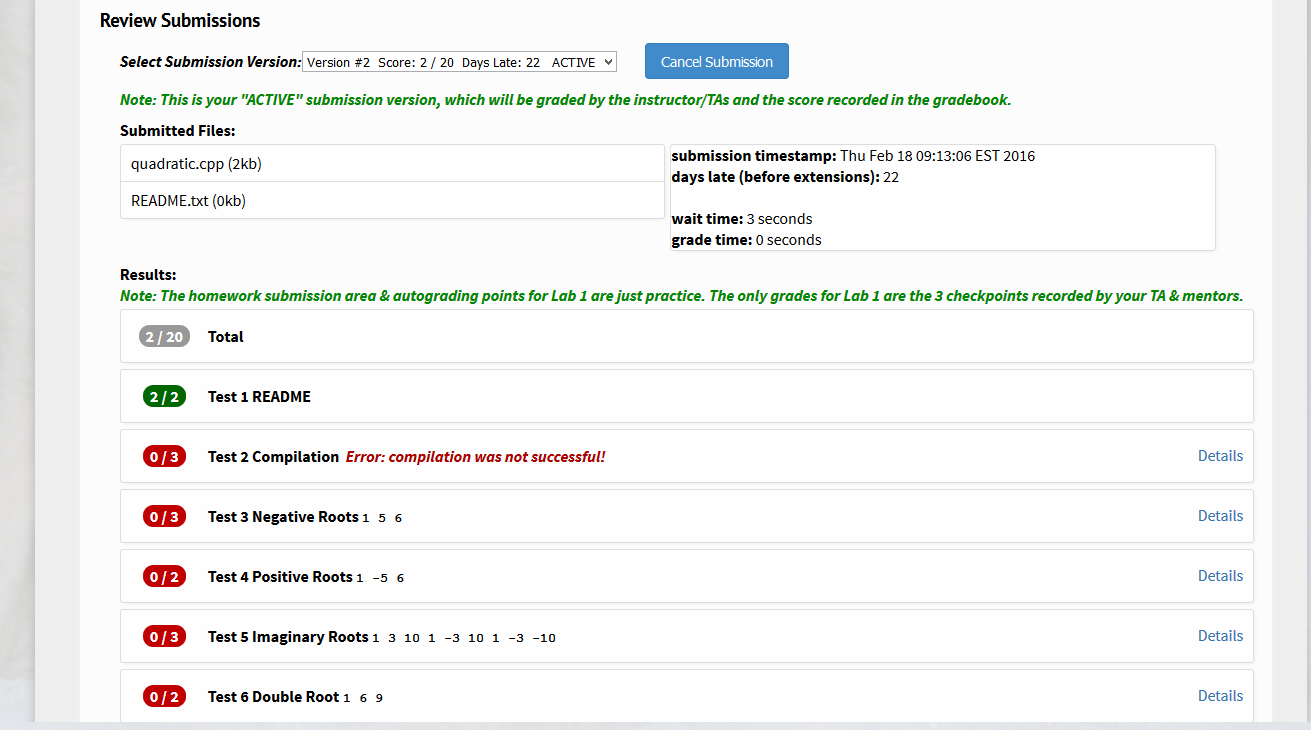
\includegraphics[width=5.8in]{CompilationError}%
\hfill
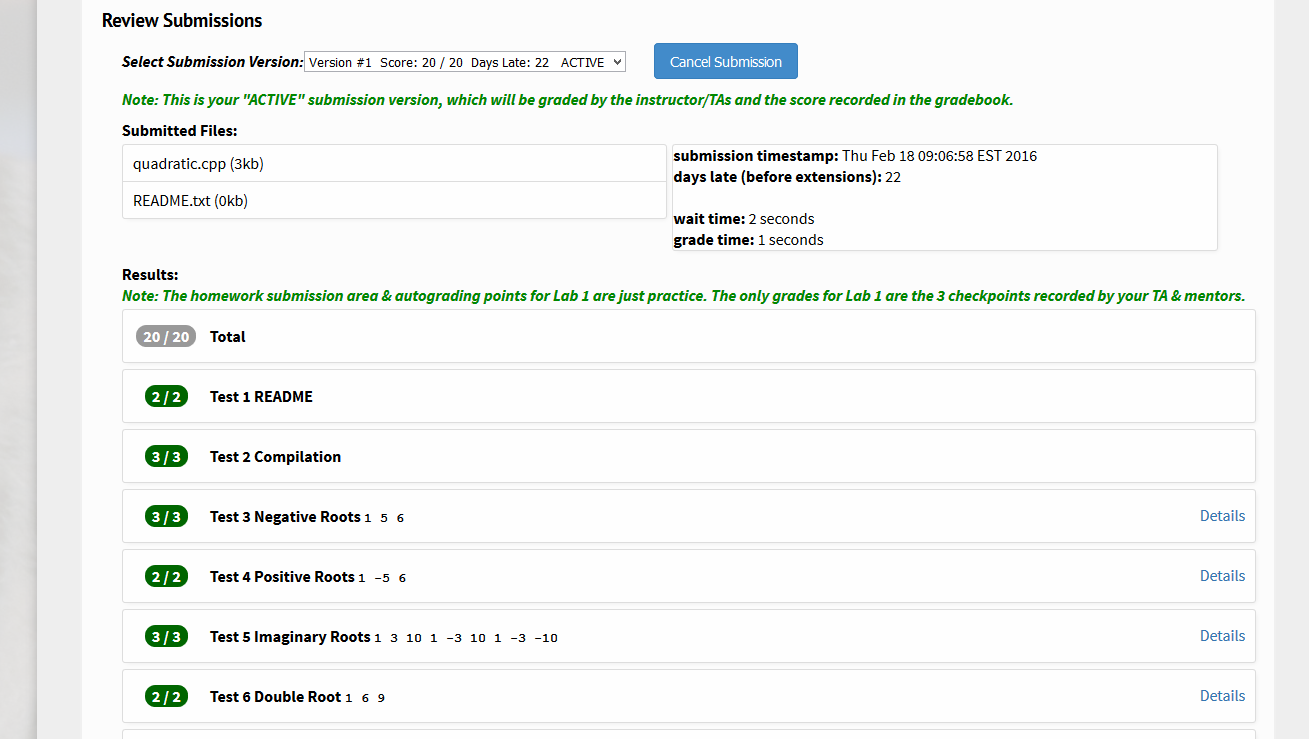
\includegraphics[width=5.8in]{AllCorrect}%
\end{center}




 \begin{itemize}   
    \item Instructors create and configure assignments for grading \\ and
customize their ``late day'' policy
    \item Website for TAs to view and grade student submissions
    \item Reduces manual TA grading - TAs do not have to manually  \\ download, build, compile, \& test submissions
    \item TAs do not have to track administrative details concerning \\ assignments (late day penalties, extensions for illness, etc.)
    \item TAs provide grades and written feedback on software quality of student homework submissions 
    \item TAs enter lab checkpoints, quiz, and test grades to the database
\end{itemize}

    \begin{center}
        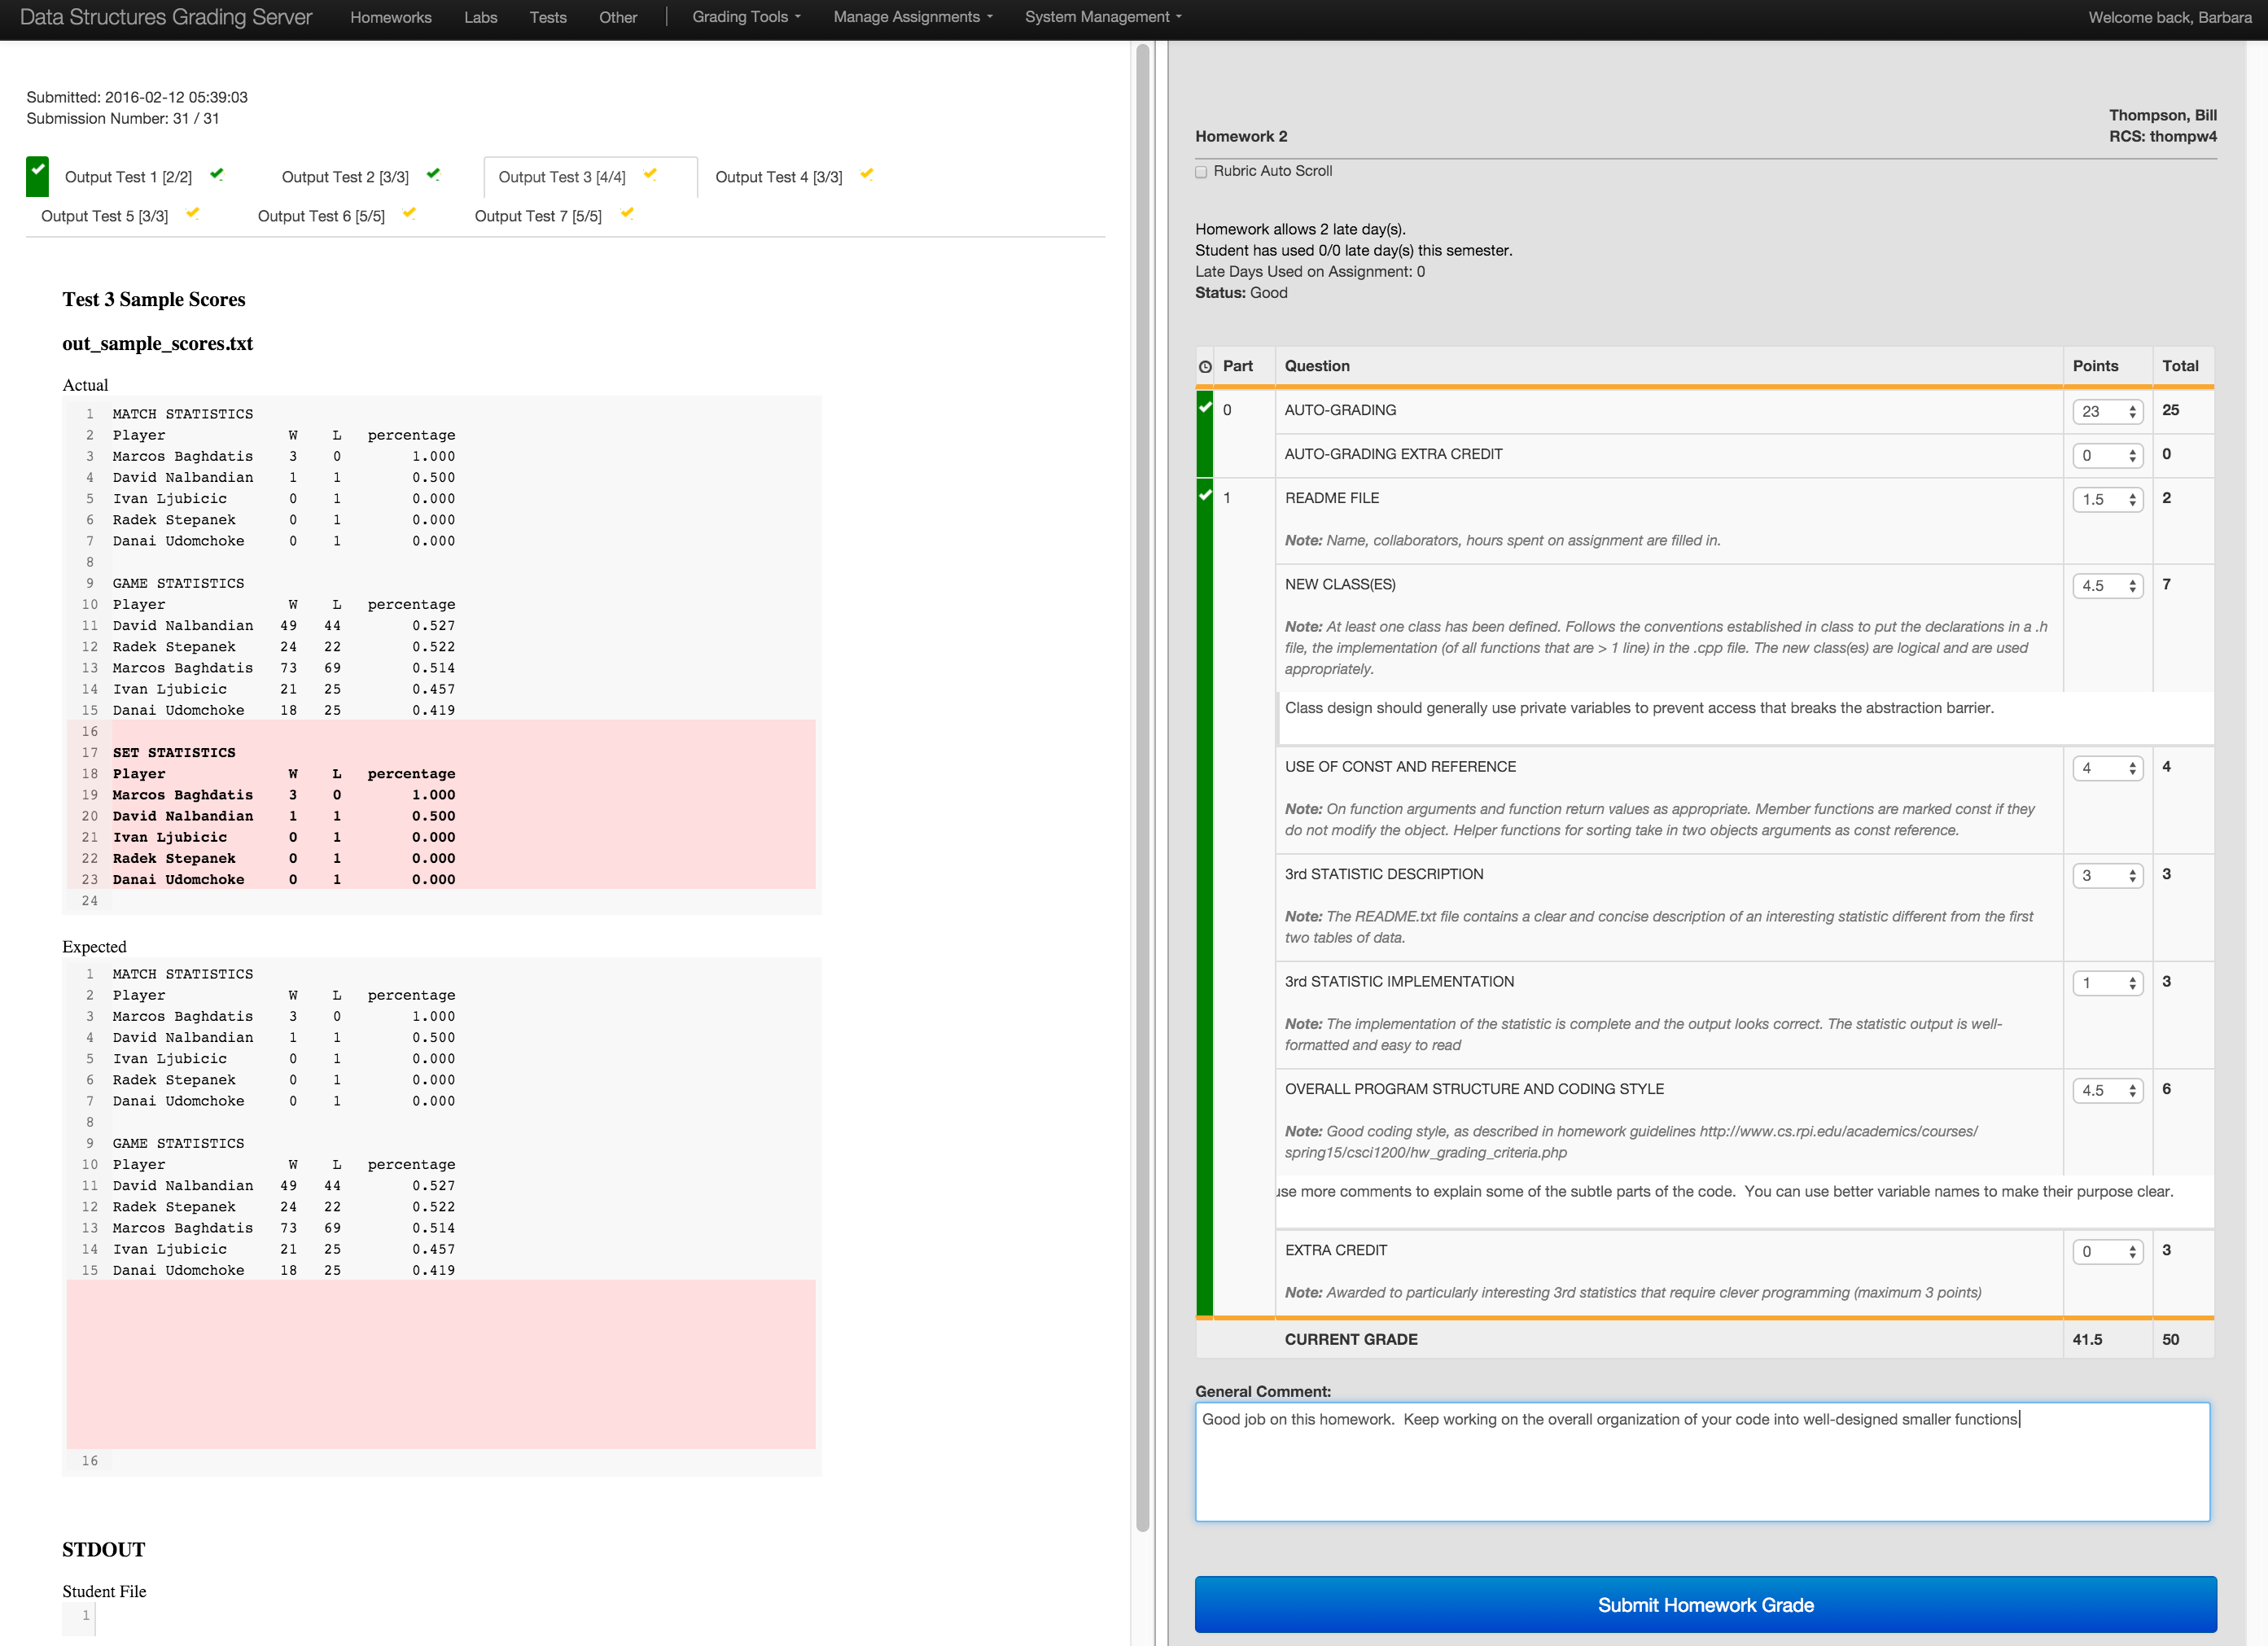
\includegraphics[width=12in]{tagrading_screenshot}
    \end{center}
        

\columnbreak

\section{3. Performance \& Robustness}%
    \begin{itemize}
        \item Multiple submissions and immediate feedback allow for an \\ interactive learning environment
        \item Ensures consistency and fairness in grading for students
        \item Little to no down time of server
        \item Runs multiple homeworks in parallel for efficient grading
        \item Server is robust - some numbers:
          \begin{itemize}
            \item 7 active courses 
            \item 14 weeks of server logs
            \item dozens of instructors \& TAs
            \item more than 1,500 students
            \item over 77,000 total submissions
    \end{itemize}
    \end{itemize}
    
\begin{center}
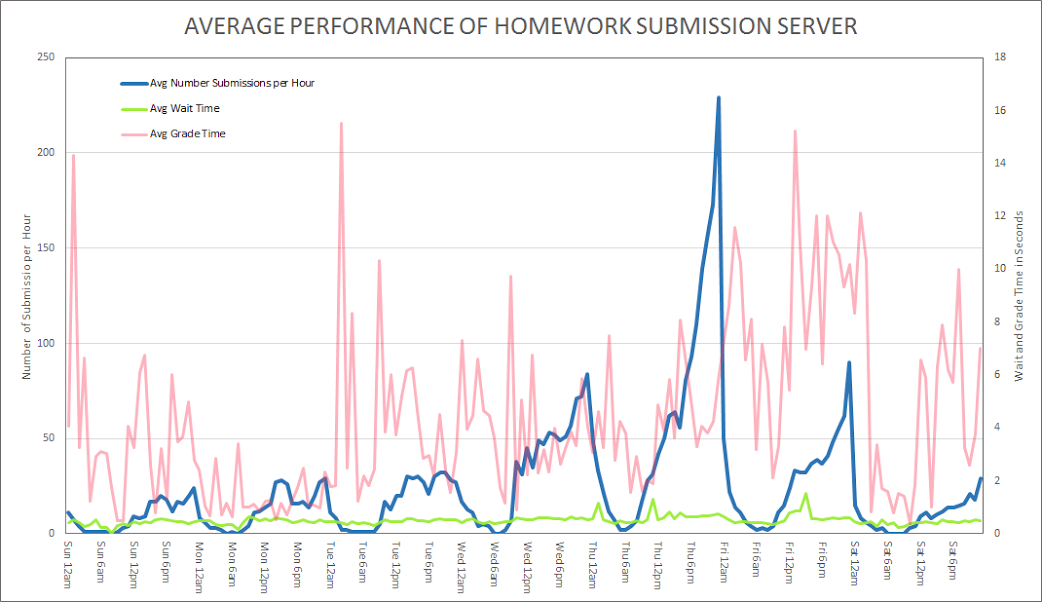
\includegraphics[width=12in]{avg_sub_wait_time}
\end{center}

\begin{center}
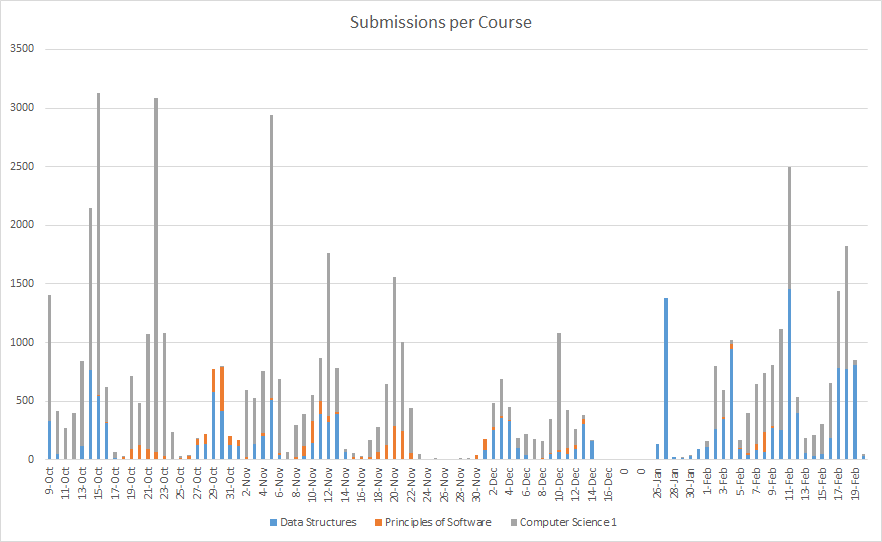
\includegraphics[width=12in]{stacked_bar_graph}
%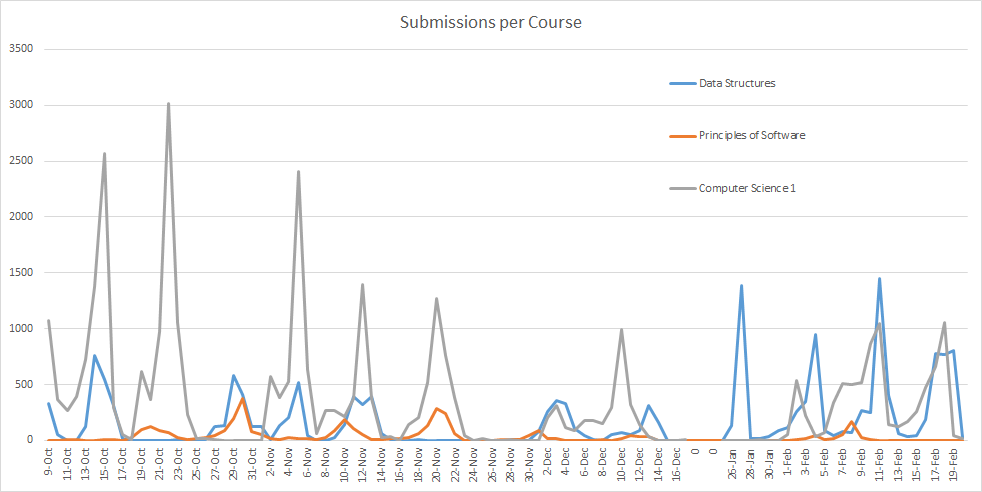
\includegraphics[width=12in]{loadperclass}
\end{center}

\columnbreak

\section{4. Survey of Students}%
%%graphs of the responses to survey questions
%%graphs of the advantages/disadvantages from survey
\begin{itemize}
    \item In mid Fall 2015, we surveyed students and TAs of the three largest courses using the server
    \item We received $\sim$400 responses from approximately 850 students
\end{itemize}

\begin{comment}
  Also received some points of criticism including:
    \begin{enumerate}
        \item "My code runs on my machine but not on the server!"
        \item How picky the server is about whitespace when comparing student and expected output
        \item Students thought run-time/compiler error messages were confusing or not helpful
    \end{enumerate}
\end{comment}


\begin{center}
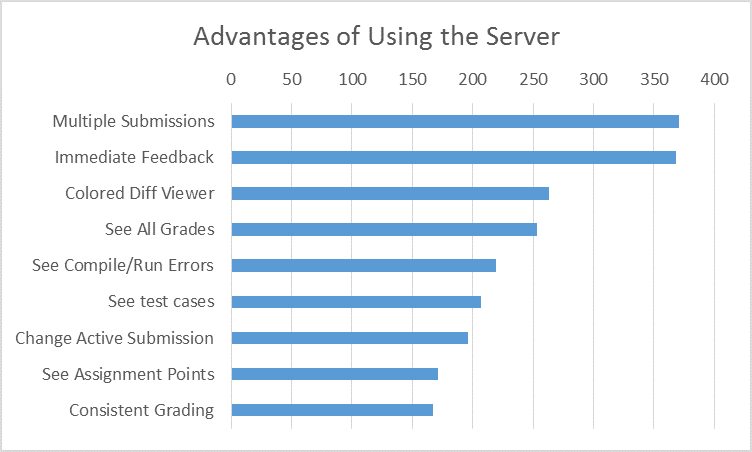
\includegraphics[width=11in]{Advantages}
\label{fig:advantages}

\vspace{0.1in}

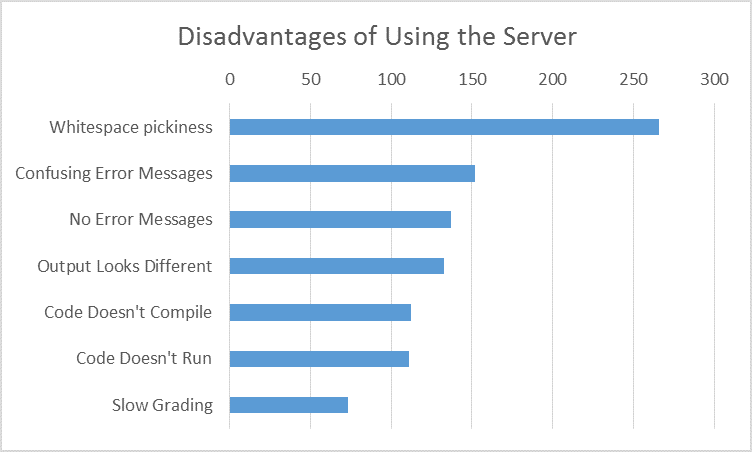
\includegraphics[width=11in]{Disadvantages}
\label{fig:disadvantages}
\end{center}

\vspace{-0.2in}

\section{5. Security}
    \begin{itemize}
        \item Database access done through the \textit{PDO library} which protects against malicious and malformed inputs
        \item 

Instructor configures appropriate \textit{resource limits} (GNU Linux {\tt rlimit}) to
{\em sandbox} testing of electronically-submitted student code and prevent issues like infinite loops, runaway output, and \\ excessive use of other system resources 

        \item Before running the student code, we switch from a privileged \\ system user to an untrusted user using GNU Linux {\tt setresuid}
        \item Careful design of file and directory permissions and database access maintains confidentiality of student work and grades
        \item Uses {\em secure computing mode} (GNU Linux {\tt seccomp}) to prevent use of sockets, fork, and other unnecessary system calls by student code
    \end{itemize}
    
\columnbreak

\section{6. Open Source Software}
    \begin{itemize}
        \item Advantages over proprietary software: \\
Free to use, no subscription required, no third-party data collection
        \item Open source can be more reliable than closed source software
        \item User interface can be improved and customized
        \item Community helps maintain codebase
        \item Improved security:  More people can study and test the software to find bugs and security vulnerabilities
    \end{itemize}

\section{7. History of the Project}%
\begin{itemize}
    \item Fall 2012: TA grading website started by TAs (closed source)
    \item January 2014: RCOS students begin development of new system
    \item Fall 2014: Rollout to first course (Data Structures)
    \item Fall 2015: TA grading website made open source 
    \item Used by: Computer Science I, Data Structures, Foundations of \\
          Computer Science, Principles of Software, Programming \\ 
          Languages, Operating Systems, Interactive Visualization, \\
          Advanced Computer Graphics, Computational Vision, \\
          Distributed Systems, and Database Systems
\end{itemize}

\section{8. Ongoing Work}%
\begin{itemize}
    \item Improve error and warning messages given to students
    \item Improve partial credit awarded for minor whitespace differences
    \item Generate and display submission statistics to the students
    \item Continued penetration testing and security improvements
    \item Improve the individual student summary grades table 
    \item Add pdf and image viewer for TA grading
    \item Expand system to additional courses in our department, to
      other departments at RPI, and to other universities
\end{itemize}

\section{9. Acknowledgments}
\begin{itemize}
    \item Red Hat Software
    \item Rensselaer Center for Open Source (RCOS)
    \item  \url{https://github.com/RCOS-Grading-Server/HWserver}
\end{itemize}

\end{poster}

\end{document}
